\documentclass[tikz,border=10pt]{standalone}
\usepackage{amsmath}
\usepackage{amssymb}
\usepackage{tikz}
\usetikzlibrary{arrows.meta,calc}

\definecolor{figazul}{RGB}{2,132,199}
\definecolor{figrojo}{RGB}{220,38,38}
\definecolor{figverde}{RGB}{22,163,74}

\begin{document}
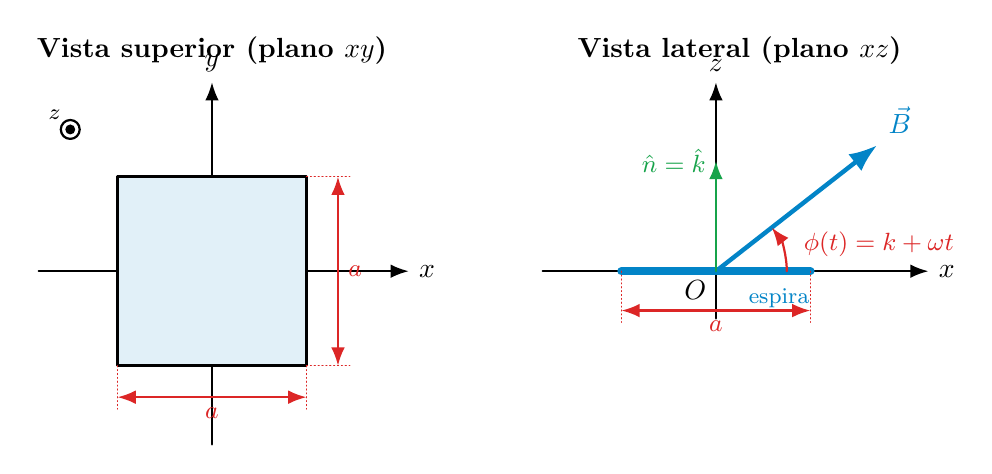
\begin{tikzpicture}[>=Latex, line cap=round, line join=round]
  % -------------------------------------------------------------
  % Panel 1: Vista superior (plano xy)
  % -------------------------------------------------------------
  \begin{scope}[xshift=0cm]
    \node[above, font=\bfseries] at (0, 2.5) {Vista superior (plano $xy$)};

    % Ejes coordenados x, y
    \draw[->, thick] (-2.2, 0) -- (2.5, 0) node[right] {$x$};
    \draw[->, thick] (0, -2.2) -- (0, 2.4) node[above] {$y$};
    \node[below left] at (0,0) {$O$};

    % Eje z saliente
    \draw[thick] (-1.8, 1.8) circle (0.12);
    \fill (-1.8, 1.8) circle (1.8pt);
    \node[above left, font=\footnotesize] at (-1.8, 1.8) {$z$};

    % Espira cuadrada de lado a = 2.4 centrada en el origen
    \draw[very thick, fill=figazul!12] (-1.2, -1.2) rectangle (1.2, 1.2);

    % Cotas de lado a
    \draw[<->, thick, color=figrojo] (-1.2, -1.6) -- (1.2, -1.6) node[midway, below, color=figrojo, font=\small] {$a$};
    \draw[densely dotted, thin, color=figrojo] (-1.2, -1.2) -- (-1.2, -1.75);
    \draw[densely dotted, thin, color=figrojo] (1.2, -1.2) -- (1.2, -1.75);

    \draw[<->, thick, color=figrojo] (1.6, -1.2) -- (1.6, 1.2) node[midway, right, color=figrojo, font=\small] {$a$};
    \draw[densely dotted, thin, color=figrojo] (1.2, -1.2) -- (1.75, -1.2);
    \draw[densely dotted, thin, color=figrojo] (1.2, 1.2) -- (1.75, 1.2);
  \end{scope}

  % -------------------------------------------------------------
  % Panel 2: Vista lateral (plano xz)
  % -------------------------------------------------------------
  \begin{scope}[xshift=6.4cm]
    \node[above, font=\bfseries] at (0.3, 2.5) {Vista lateral (plano $xz$)};

    % Ejes coordenados x, z
    \draw[->, thick] (-2.2, 0) -- (2.7, 0) node[right] {$x$};
    \draw[->, thick] (0, -0.6) -- (0, 2.4) node[above] {$z$};
    \node[below left] at (0,0) {$O$};

    % Espira vista de perfil (en el plano z=0, entre -1.2 y 1.2)
    \draw[line width=3pt, color=figazul] (-1.2, 0) -- (1.2, 0);
    \node[below, font=\footnotesize, color=figazul] at (0.8, -0.1) {espira};

    % Campo magnético B con ángulo de elevación \phi respecto a +x
    \draw[->, ultra thick, color=figazul] (0, 0) -- (38:2.6) node[above right, color=figazul] {$\vec{B}$};

    % Arco del ángulo phi(t) = k + \omega t
    \draw[->, thick, color=figrojo] (0.9, 0) arc (0:38:0.9);
    \node[right, color=figrojo, font=\small] at (19:1.05) {$\phi(t) = k + \omega t$};

    % Vector normal n_hat = z_hat
    \draw[->, thick, color=figverde] (0, 0) -- (0, 1.4) node[left, color=figverde, font=\small] {$\hat{n} = \hat{k}$};

    % Cota de ancho a
    \draw[<->, thick, color=figrojo] (-1.2, -0.5) -- (1.2, -0.5) node[midway, below, color=figrojo, font=\small] {$a$};
    \draw[densely dotted, thin, color=figrojo] (-1.2, 0) -- (-1.2, -0.65);
    \draw[densely dotted, thin, color=figrojo] (1.2, 0) -- (1.2, -0.65);
  \end{scope}
\end{tikzpicture}
\end{document}
